\documentclass{article}
\usepackage[utf8]{inputenc}
\usepackage[T1]{fontenc}
\usepackage{csvsimple}
\usepackage{rotating}
\usepackage{graphicx}
\usepackage{amsmath}
\usepackage{listings}
\setlength{\parindent}{0pt}
\title{Symulacje Monte Carlo}
\date{}

\begin{document}

\maketitle
Temat: \textbf{Model Isinga 2D}\\
Imię i nazwisko prowadzącego: \textbf{Grzegorz Pawlik}

\begin{center}
\begin{tabular}{|p{5cm}|p{6cm}|}
\hline
$Wykonawca:$ & $Gracjan$ $Tokarz$ $255531$ $W11$  \\
\hline
$Termin$ $zajec:$ & $Piatek , 15:15$\\
\hline
$Data$ $oddania$ $sprawozdania:$ & $15.01.2021r$\\
\hline
\textbf{Ocena	końcowa:} & \\
\hline
\end{tabular}
\end{center}

\textbf{Adnotacje dotyczące wymaganych poprawek,oraz daty otrzymania poprawionego sprawozdania}

\newpage

\section{Kod źródłowy}

\lstset{
	language=C++
}
\begin{lstlisting}[basicstyle=\small]

#include <stdio.h>
#include <math.h>
#include <stdlib.h>
#include <time.h>
#define N 200

float calcX(int index, float unit);
float calcV(float x);
void energyToFile(float E, int step);
void phiToFile(float phi, float x, float denominator, float unit);
float set(float phi, float dphi);

int main(){
	float unit = (float) 8 / N;
	int steps = 1000000000;
        int index;
	float phiStart = 0.1;
	float dPhi = 0.1;
	float phi[N+1]; 
	float U = 0, T = 0, denominator = 0, numerator, E, r, phiTrial;
	for (int i = 0; i <= N; i++) {//setting phi and U
		phi[i] = phiStart;
		U += (phi[i] * phi[i] * calcV( calcX(i, unit) ));
		denominator += phi[i] * phi[i];
	}

	for (int i = 1; i < N; i++){
	       	T += 0.5 * phi[i] * (2 * phi[i] - phi[i-1] - phi[i+1]);
	}
	T +=0.5*phi[0] * (2 * phi[0] - phi[1]);
	T += 0.5*phi[N] * (2 * phi[N] - phi[N-1]);
	T = T / (unit * unit);//kinetic energy
	numerator = U + T;
	E = numerator / denominator;//starting energy
	float deltaPhi, dU,dT, deltaPhiSqr, newE;











	for (int i = 0; i <= steps; i++){
		r = (float)rand()/RAND_MAX;
		index = rand() % N;
		phiTrial = phi[index] + (r - 0.5)*dPhi;
		deltaPhi = phiTrial - phi[index];
		deltaPhiSqr = phiTrial * phiTrial - phi[index] * phi[index];
		if (index == 0) dT = deltaPhiSqr - deltaPhi * phi[index+1];
		else if (index == N) dT = deltaPhiSqr - deltaPhi * phi[index-1];
		else dT = deltaPhiSqr  - deltaPhi * (phi[index+1] + phi[index-1]);
		dT = dT / (unit*unit);
		dU = deltaPhiSqr * calcV( calcX(index, unit) );
		newE = (numerator + dU + dT) / (denominator + deltaPhiSqr);
		if (newE < E && newE > 0){
			phi[index] = phiTrial;
			E = newE;
			numerator += dU + dT;
			denominator += deltaPhiSqr;
		}
		if(i%100000==0) energyToFile(E, i);
	}
	for (int i = 0; i <= N;i++){
		phiToFile(phi[i], calcX(i, unit), denominator, unit );
	}
	return 0;
}
void phiToFile(float phi, float x, float denominator, float unit){
	FILE *file;
	file = fopen("phi.dat","a+");
	float phiNorm = phi/sqrt(denominator*unit);
	fprintf(file,"%f\t%f\n",x, phiNorm);
	fclose(file);
}
void energyToFile(float E, int step){
	FILE *file;
	file = fopen("energy.dat","a+");
	fprintf(file, "%f\t%d\n",step, E);
	fclose(file);
}
float calcV (float x){
	return 0.5*x*x;
}
float calcX(int index, float unit){
	if (index > N || index < 0){
		printf("%d - wrong index - out of scope\n", index);
		return 10;
	}
	else return (-4 + (index * unit));
}

\end{lstlisting}

\newpage
\section{Wyniki obliczeń i parametry symulacji}
\begin{center}
\begin{tabular}{p{5cm}|p{5cm}}
	Energia końcowa: & $0.540255$\\
	\hline
	Ilość kroków MC: & $1 000 000 000$\\
	\hline
	$\varphi$ początkowe: & $0.1$\\
	\hline
	$\Delta \varphi:$ & $0.1$\\
	\hline
	Czynnik normujący: & $1.8861648$\\
\end{tabular}
\end{center}

\section{Wykresy}
\subsection{Wykres unormowanej funkcji falowej}
%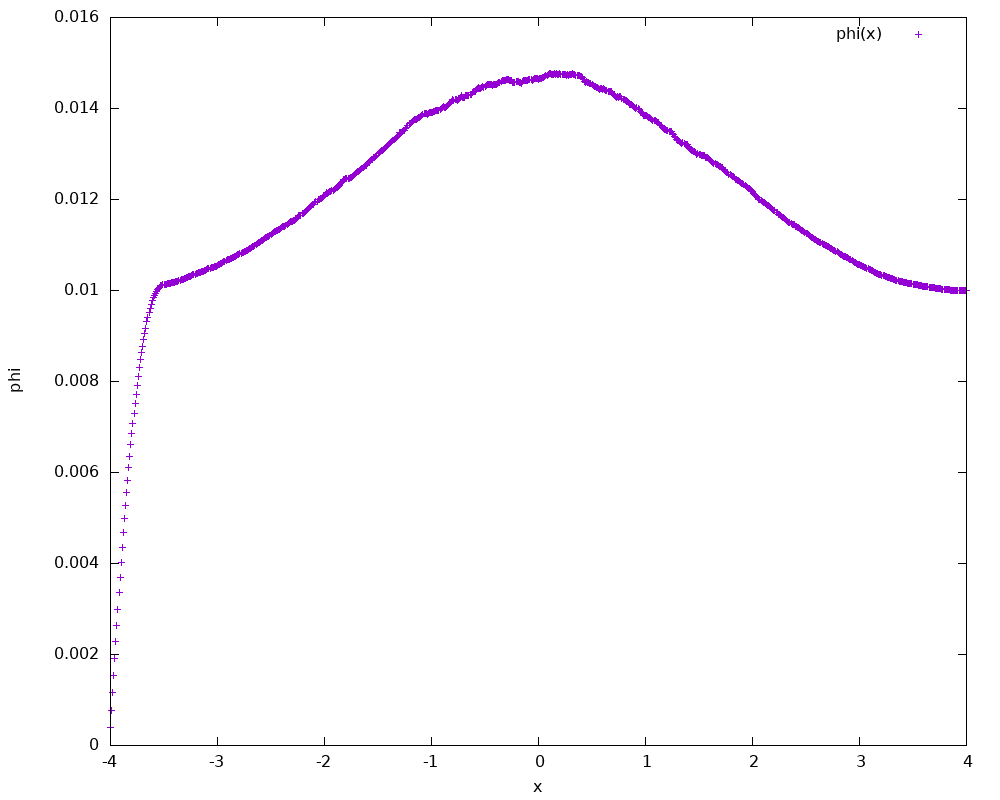
\includegraphics[width=13cm]{phi.png}

\subsection{Wykres unergii układu w toku symulacji}
%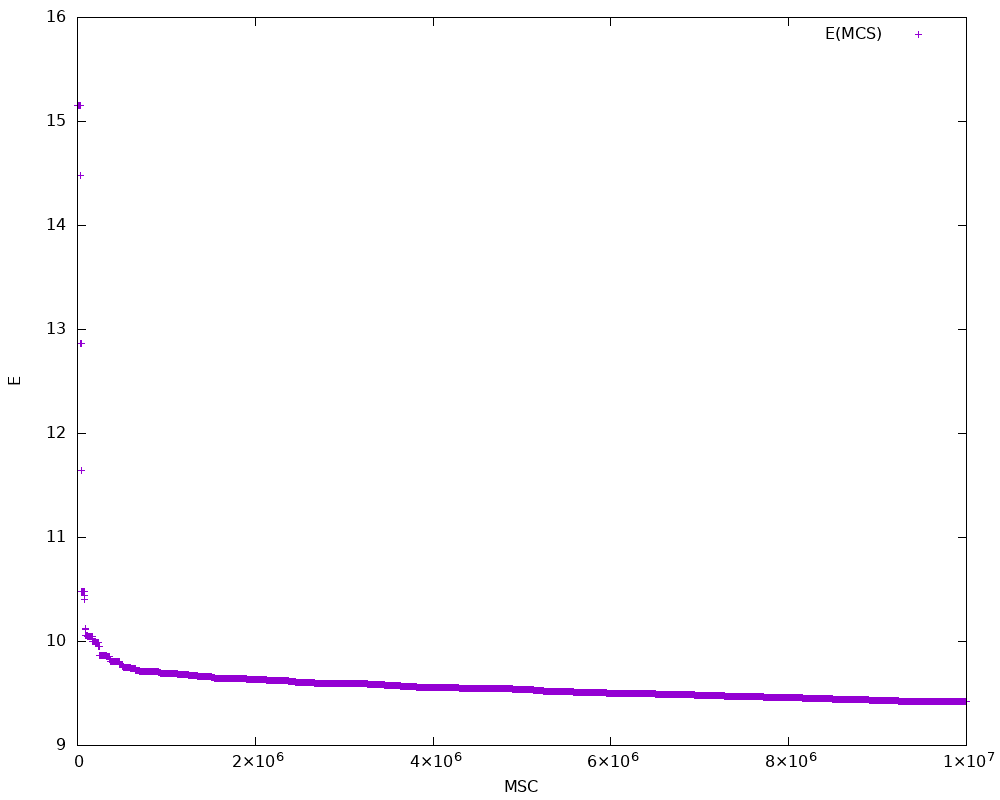
\includegraphics[width=13cm]{energy.png}

\end{document}
